\documentclass[aspectratio=43, xcolor=table]{beamer}
%\usepackage[english]{babel}

%Cargar paquetes
\usepackage[utf8]{inputenc}%Permite usar acentos
\usepackage[spanish]{babel}%Configura el idioma por defecto a español
\usepackage{amsmath}%Introduce términos matemáticos
\usepackage{graphicx}%Permite introducir figuras
\usepackage[options]{natbib}%Bibliografía con estilos %No funcionan estilos en Beamer
\newcommand{\grad}{\hspace{-2mm}$\phantom{a}^{\circ}$}

\usepackage{amsthm}
\usepackage{mathtools}
\usepackage{physics}
\usepackage{calligra}
\usepackage{csquotes}
\usepackage{tensor}
\usepackage[thicklines]{cancel}
\usepackage{tcolorbox}
\usepackage{pstricks}
\usepackage[backend=biber, bibstyle=nature, sorting=nty, citestyle=numeric-comp]{biblatex} %Custom bibliography
    \addbibresource{bib.bib} %Load references


\DeclareMathAlphabet{\mathcalligra}{T1}{calligra}{m}{n}
\DeclareFontShape{T1}{calligra}{m}{n}{<->s*[2.2]callig15}{}
\newcommand{\scriptr}{\mathcalligra{r}\,}
\newcommand{\boldscriptr}{\pmb{\mathcalligra{r}}\,}
\def\rc{\scriptr}
\def\brc{\boldscriptr}
\def\hrc{\hat\brc}
\newcommand{\ie}{\emph{i.e.}} %id est
\newcommand{\eg}{\emph{e.g.}} %exempli gratia
\newcommand{\rtd}[1]{\ensuremath{\left\lfloor #1 \right\rfloor}}
\newcommand{\dirac}[1]{\ensuremath{\delta \left( #1 \right)}}
\newcommand{\diract}[1]{\ensuremath{\delta^3 \left( #1 \right)}}
\newcommand{\e}{\ensuremath{\epsilon_0}}
\newcommand{\m}{\ensuremath{\mu_0}}
\newcommand{\V}{\ensuremath{\mathcal{V}}}
\newcommand{\prnt}[1]{\ensuremath{\left(#1\right)}} %parentheses
\newcommand{\colch}[1]{\ensuremath{\left[#1\right]}} %square brackets
\newcommand{\chave}[1]{\ensuremath{\left\{#1\right\}}}  %curly brackets

\useoutertheme{infolines}
\useinnertheme{rectangles}
\usefonttheme{professionalfonts}


\definecolor{orange}{HTML}{f28165}
\definecolor{gray}{HTML}{303030}
\definecolor{yellow}{HTML}{f0be52}
\definecolor{lightorange}{HTML}{f19e58}

\renewcommand{\CancelColor}{\color{orange}}

\makeatletter
\newcommand{\mybox}[1]{%
  \setbox0=\hbox{#1}%
  \setlength{\@tempdima}{\dimexpr\wd0+13pt}%
  \begin{tcolorbox}[colback=orange,colframe=orange,boxrule=0.5pt,arc=4pt,
      left=6pt,right=6pt,top=6pt,bottom=6pt,boxsep=0pt,width=\@tempdima]
    \textcolor{white}{#1}
  \end{tcolorbox}
}
\makeatother

\usecolortheme[named=orange]{structure}
\usecolortheme{sidebartab}
\usecolortheme{orchid}
\usecolortheme{whale}
\setbeamercolor{alerted text}{fg=yellow}
\setbeamercolor{block title alerted}{bg=alerted text.fg!90!black}
\setbeamercolor{block title example}{bg=lightorange!60!black}
\setbeamercolor{background canvas}{bg=gray}
\setbeamercolor{normal text}{bg=gray,fg=white}

\setbeamertemplate{footline}
        {
      \leavevmode%
      \hbox{%
      \begin{beamercolorbox}[wd=.333333\paperwidth,ht=2.25ex,dp=1ex,center]{author in head/foot}%
        \usebeamerfont{author in head/foot}\insertshortauthor~~(\insertshortinstitute)
      \end{beamercolorbox}%
      \begin{beamercolorbox}[wd=.333333\paperwidth,ht=2.25ex,dp=1ex,center]{title in head/foot}%
        \usebeamerfont{title in head/foot}\insertshorttitle
      \end{beamercolorbox}%
      \begin{beamercolorbox}[wd=.333333\paperwidth,ht=2.25ex,dp=1ex,center]{date in head/foot}%
        \usebeamerfont{page number in head/foot}\insertframenumber/\inserttotalframenumber%\hspace*{2em}

    %#turning the next line into a comment, erases the frame numbers
        %\insertframenumber{} / \inserttotalframenumber\hspace*{2ex} 

      \end{beamercolorbox}}%
      \vskip0pt%
    }


\setbeamertemplate{blocks}[rectangle]
\setbeamercovered{dynamic}

\setbeamertemplate{section page}
{
	\begin{centering}
		\begin{beamercolorbox}[sep=27pt,center]{part title}
			\usebeamerfont{section title}\insertsection\par
			\usebeamerfont{subsection title}\insertsubsection\par
		\end{beamercolorbox}
	\end{centering}
}

%\setbeamertemplate{subsection page}
%{
%	\begin{centering}
%		\begin{beamercolorbox}[sep=12pt,center]{part title}
%			\usebeamerfont{subsection title}\insertsubsection\par
%		\end{beamercolorbox}
%	\end{centering}
%}

\newcommand{\hlight}[1]{\colorbox{violet!50}{#1}}
\newcommand{\hlighta}[1]{\colorbox{red!50}{#1}}
\title{Simulación manual} %->->->->-> Check hyperref title <-<-<-<-<-
%\subtitle{And Some Things About It}
\author[C.J. Uribe-Martes]{Carlos Javier Uribe Martes}
\institute[CUC]{
    Ingeniería Industrial%
    \\%
    Universidad de la Costa%
} %You can change the Institution if you are from somewhere else
\date{Febrero 22, 2020}
%\logo{\includegraphics[width= 0.2\textwidth]{images/a-logo.png}}

\begin{document}
    
    \frame{\titlepage}
    
    \begin{frame}{Contenido}
        \tableofcontents
    \end{frame}
    
    \section{Simulación manual}

\begin{frame}{Simulación de eventos discretos}
    \begin{itemize}
        \item Aunque la simulación por eventos discretos puede conceptualmente realizarse a mano, la cantidad de datos que deben almacenarse y manipularse para la mayoría de las aplicaciones reales involucra el uso de un computador.
    \end{itemize}
\end{frame}

\begin{frame}{Simulación manual}{Reloj de la simulación}
    \begin{itemize}
        \item Dada la naturaleza dinámica de los modelos de simulación por eventos discretos, se requiere hacer seguimiento del valor actual del \textit{tiempo simulado}.
        \item De igual forma, se requiere un mecanismo para avanzar el tiempo simulado de un valor a otro.
        \item La variable dentro de un modelo de simulación que guarda el valor actual del tiempo simulado se llama \textit{reloj de la simulación}.
    \end{itemize}
\end{frame}

\begin{frame}{¿Cómo empezar a simular?}
    \begin{itemize}
        \item Hasta que se encuentre cómodo con sus competencias de modelado se recomienda responder a las siguientes preguntas:
        \begin{itemize}
            \item ¿Cuál es el sistema? ¿Qué información se conoce del sistema?
            \item ¿Cuáles son las medidas de desempeños requeridas?
            \item ¿Cuáles son las entidades? ¿Qué información debe ser almacenada o tenida en cuenta para cada entidad? ¿Cómo ingresas las entidades al sistema?
            \item ¿Cuáles son los recursos que utilizan las entidades? ¿Qué entidades usan cuáles recursos y cómo?
            \item ¿Cuáles son los flujos del proceso? Diagrame el flujo del proceso o un diagrama de actividad preliminar.
            \item Desarrolle un pseudo-código para el modelo o un modelo conceptual completo.
        \end{itemize}
    \end{itemize}
\end{frame}

\begin{frame}{Simulación manual}
    \begin{itemize}
        \item El analista debe definir:
        \begin{enumerate}
            \item Entradas: Parámetros exógenos que, usualmente, son independientes de otras características del sistema.
            \item Salidas: Valores utilizados para calcular las medidas de desempeño del sistema (respuestas o indicadores).
            \item Estados del sistema: Conjunto de variables de estado que definen el sistema en un momento dado.
        \end{enumerate}
    \end{itemize}
\end{frame}

\begin{frame}{Pasos para realizar una simulación manual}
    \begin{itemize}
        \item Se recomienda al analista seguir estas pautas:
        \begin{enumerate}
            \item Determine las características de cada entrada.
            \item Determine las actividades, eventos y estados del sistema relevantes.
            \item Determine el resumen de las medidas de desempeño requeridas.
            \item Determinar las salidas requeridas para calcular las medidas de desempeño.
            \item Construir una tabla de simulación.
            \item En cada paso, genere un valor para las actividades, encuentre los estados del sistema y calcule las salidas.
            \item Cuando termine la simulación, utilice las salidas para calcular las medidas de desempeño.
        \end{enumerate}
    \end{itemize}
\end{frame}

\begin{frame}{Tablas de simulación}
    \begin{itemize}
        \item Se diseña de forma tal que cada paso dependa únicamente de entradas del modelo o de uno o varios pasos o valores previamente computados.
    \end{itemize}
\end{frame}

\begin{frame}{Tablas de simulación}{Columnas}
    \begin{itemize}
        \item Cada columna puede contener:
        \begin{enumerate}
            \item Una actividad asociada con una entrada del modelo.
            \item Una variable aleatoria definida como una entrada del modelo.
            \item Un estado del sistema.
            \item Un evento, o la hora del reloj de un evento.
            \item Una salida del modelo.
            \item Una respuesta o indicador.
        \end{enumerate}
    \end{itemize}
\end{frame}

\begin{frame}{Tablas de simulación}{Filas}
    \begin{itemize}
        \item Cada fila puede representar:
        \begin{enumerate}
            \item La ocurrencia de uno o más eventos.
            \item El progreso de una entidad a través del sistema.
        \end{enumerate}
    \end{itemize}
\end{frame}

\begin{frame}{Uso de aleatorios}
    \begin{itemize}
        \item Es una buena práctica utilizar una secuencia de aleatorios y continuar de una manera sistemática, sin utilizar más de una vez la misma secuencia en un problema dado.
        \item Si la misma secuencia es usada de forma repetida, pueden ocurrir sesgos estadísticos u otros efectos no deseados que afecten los resultados.
    \end{itemize}
\end{frame}
    
    \section{Modelos de colas}

\begin{frame}{Simulación de un modelo de colas}
    \begin{itemize}
        \item Los estados del sistema de un modelo de colas consisten en el número de unidades en el sistema y el estado del sistema (ocupado o desocupado).
        \item Los eventos típicos representan la llegada de un nuevo cliente, el inicio de la atención y la salida de un cliente.
    \end{itemize}
\end{frame}

\begin{frame}{Tabla de simulación para un modelo de colas}
    \begin{itemize}
        \item La simulación de colas requiere conservar una lista de eventos para determinar qué sigue a continuación, llamada \textit{calendario de eventos}.
    \end{itemize}
\end{frame}


\begin{frame}{Tabla de simulación para un modelo de colas}
\begin{table}[]
\begin{tabular}{|c|c|c|c|c|c|}
\hline
\rowcolor[HTML]{794033} 
{\color[HTML]{FFFFFF} \textbf{\begin{tabular}[c]{@{}c@{}}Cliente\\ número\end{tabular}}} & {\color[HTML]{FFFFFF} \textbf{\begin{tabular}[c]{@{}c@{}}T. entre\\ llegada\\ (activ.)\end{tabular}}} & {\color[HTML]{FFFFFF} \textbf{\begin{tabular}[c]{@{}c@{}}Hora\\ llegada\\ (reloj)\end{tabular}}} & {\color[HTML]{FFFFFF} \textbf{\begin{tabular}[c]{@{}c@{}}Hora inicio\\ servicio \\ (reloj)\end{tabular}}} & {\color[HTML]{FFFFFF} \textbf{\begin{tabular}[c]{@{}c@{}}T. de\\ servicio\\ (activ.)\end{tabular}}} & {\color[HTML]{FFFFFF} \textbf{\begin{tabular}[c]{@{}c@{}}Hora fin\\ servicio\\ (reloj)\end{tabular}}} \\ \hline
\rowcolor[HTML]{F28165} 
{\color[HTML]{FFFFFF} 1} & {\color[HTML]{FFFFFF} 0}  & {\color[HTML]{FFFFFF} 0} & {\color[HTML]{FFFFFF} 0} & {\color[HTML]{FFFFFF} 2} & {\color[HTML]{FFFFFF} 2} \\ \hline
\rowcolor[HTML]{F28165} 
{\color[HTML]{FFFFFF} 2} & {\color[HTML]{FFFFFF} 2} & {\color[HTML]{FFFFFF} 2} & {\color[HTML]{FFFFFF} 2} & {\color[HTML]{FFFFFF} 1} & {\color[HTML]{FFFFFF} 3} \\ \hline
\rowcolor[HTML]{F28165} 
{\color[HTML]{FFFFFF} 3} & {\color[HTML]{FFFFFF} 4} & {\color[HTML]{FFFFFF} 6} & {\color[HTML]{FFFFFF} 6} & {\color[HTML]{FFFFFF} 3} & {\color[HTML]{FFFFFF} 9} \\ \hline
\rowcolor[HTML]{F28165} 
{\color[HTML]{FFFFFF} 4} & {\color[HTML]{FFFFFF} 1} & {\color[HTML]{FFFFFF} 7} & {\color[HTML]{FFFFFF} 9} & {\color[HTML]{FFFFFF} 2} & {\color[HTML]{FFFFFF} 11} \\ \hline
\rowcolor[HTML]{F28165} 
{\color[HTML]{FFFFFF} 5} & {\color[HTML]{FFFFFF} 2} & {\color[HTML]{FFFFFF} 9} & {\color[HTML]{FFFFFF} 11} & {\color[HTML]{FFFFFF} 1} & {\color[HTML]{FFFFFF} 12} \\ \hline
\rowcolor[HTML]{F28165} 
{\color[HTML]{FFFFFF} 6} & {\color[HTML]{FFFFFF} 6} & {\color[HTML]{FFFFFF} 15} & {\color[HTML]{FFFFFF} 15} & {\color[HTML]{FFFFFF} 4} & {\color[HTML]{FFFFFF} 19} \\ \hline
\end{tabular}
\end{table}
\end{frame}

\begin{frame}{Calendario de eventos}
% Please add the following required packages to your document preamble:
% \usepackage[table,xcdraw]{xcolor}
% If you use beamer only pass "xcolor=table" option, i.e. \documentclass[xcolor=table]{beamer}
\begin{table}[]
\begin{tabular}{|l|c|c|}
\hline
\rowcolor[HTML]{794033} 
{\color[HTML]{FFFFFF} \textbf{Evento}} & \multicolumn{1}{l|}{\cellcolor[HTML]{794033}{\color[HTML]{FFFFFF} \textbf{\begin{tabular}[c]{@{}l@{}}Cliente\\ número\end{tabular}}}} & \multicolumn{1}{l|}{\cellcolor[HTML]{794033}{\color[HTML]{FFFFFF} \textbf{\begin{tabular}[c]{@{}l@{}}Hora del\\ reloj\end{tabular}}}} \\ \hline
\rowcolor[HTML]{F28165} 
{\color[HTML]{FFFFFF} Llegada} & {\color[HTML]{FFFFFF} 1} & {\color[HTML]{FFFFFF} 0} \\ \hline
\rowcolor[HTML]{F28165} 
{\color[HTML]{FFFFFF} Salida} & {\color[HTML]{FFFFFF} 1} & {\color[HTML]{FFFFFF} 2} \\ \hline
\rowcolor[HTML]{F28165} 
{\color[HTML]{FFFFFF} Llegada} & {\color[HTML]{FFFFFF} 2} & {\color[HTML]{FFFFFF} 2} \\ \hline
\rowcolor[HTML]{F28165} 
{\color[HTML]{FFFFFF} Salida} & {\color[HTML]{FFFFFF} 2} & {\color[HTML]{FFFFFF} 3} \\ \hline
\rowcolor[HTML]{F28165} 
{\color[HTML]{FFFFFF} Llegada} & {\color[HTML]{FFFFFF} 3} & {\color[HTML]{FFFFFF} 6} \\ \hline
\rowcolor[HTML]{F28165} 
{\color[HTML]{FFFFFF} Llegada} & {\color[HTML]{FFFFFF} 4} & {\color[HTML]{FFFFFF} 7} \\ \hline
\rowcolor[HTML]{F28165} 
{\color[HTML]{FFFFFF} Salida} & {\color[HTML]{FFFFFF} 3} & {\color[HTML]{FFFFFF} 9} \\ \hline
\rowcolor[HTML]{F28165} 
{\color[HTML]{FFFFFF} Llegada} & {\color[HTML]{FFFFFF} 5} & {\color[HTML]{FFFFFF} 9} \\ \hline
\rowcolor[HTML]{F28165} 
{\color[HTML]{FFFFFF} Salida} & {\color[HTML]{FFFFFF} 4} & {\color[HTML]{FFFFFF} 11} \\ \hline
\rowcolor[HTML]{F28165} 
{\color[HTML]{FFFFFF} Salida} & {\color[HTML]{FFFFFF} 5} & {\color[HTML]{FFFFFF} 12} \\ \hline
\rowcolor[HTML]{F28165} 
{\color[HTML]{FFFFFF} Llegada} & {\color[HTML]{FFFFFF} 6} & {\color[HTML]{FFFFFF} 15} \\ \hline
\rowcolor[HTML]{F28165} 
{\color[HTML]{FFFFFF} Salida} & {\color[HTML]{FFFFFF} 6} & {\color[HTML]{FFFFFF} 19} \\ \hline
\end{tabular}
\end{table}
\end{frame}

\begin{frame}{Medidas de desempeño}
\begin{itemize}
    \item Algunas de las medidas de desempeño de interés son:
\end{itemize}
\[\text{T. promedio de espera}=\frac{\text{T. total de espera de los clientes}}{\text{Número total de clientes}}\]
\[\text{Probabilidad de esperar}=\frac{\text{Número de clientes que esperan}}{\text{Número total de clientes}}\]
\[\text{Utilización del servidor}=\frac{\text{T. total que el servidor está ocupado}}{\text{T. total de la simulación}}\]
\[\text{T. promedio de los clientes en fila}=\frac{\text{T. total de espera de los clientes}}{\text{No. total de clientes que esperan}}\]
\[\text{T. promedio en el sistema}=\frac{\text{T. total de los clientes en el sistema}}{\text{No. total de clientes}}\]
\end{frame}

    
    \section{Modelos de inventario}

\begin{frame}{Simulación de un modelo de inventarios}
    \begin{itemize}
        \item Los estados del sistema se refieren al nivel de inventario actual, pedidos pendientes, existencia de \textit{backorders}.
        \item Los eventos que pueden ocurrir se relacionan con la demanda de unidades del inventario, la revisión de la posición del inventario y la decisión resultante de hacer una orden y la llegada de un pedido.
    \end{itemize}
\end{frame}

\begin{frame}{Sistema de inventarios $(s,S)$}
    \begin{itemize}
        \item Una política de inventarios $(s,S)$, es un sistema de revisión continua.
        \item Si el inventario se encuentra en un nivel igual o menor que $s$ se solicitan suficientes unidades para llevar el inventario a un nivel $S$.
        \item El \textit{lead time}, $l$, puede ser variable.
        \item La demanda por lo general no se conoce con certeza, por lo que puede modelarse a través de una variable aleatoria.
        \item Puede o no admitirse la ocurrencia de \textit{backorders}.
    \end{itemize}
\end{frame}

\begin{frame}{Sistema de inventarios $(s,S)$}
    \begin{figure}
        \centering
        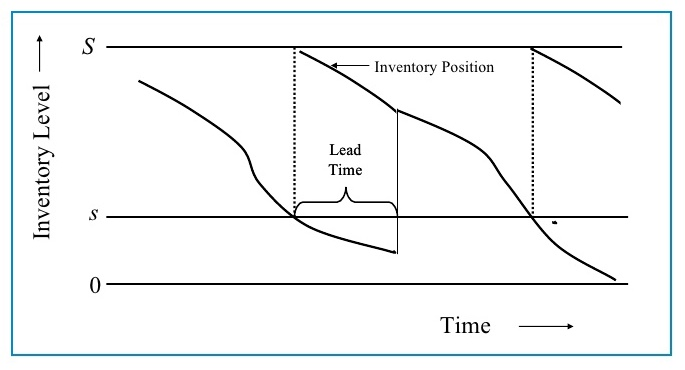
\includegraphics[width=10cm]{images/inventory-management12248440536560389-73-728-2.jpg}
        %\caption{Caption}
        \label{fig:my_label}
    \end{figure}
\end{frame}

\begin{frame}{Parámetros de interés}
    \begin{itemize}
        \item Las políticas de inventario tienen varios parámetros, algunos controlables y otros no.
        \item Entre los parámetros controlables se encuentran:
        \begin{itemize}
            \item Inventario máximo, $S$.
            \item Inventario de seguridad, $s$.
            \item Lead time, $l$.
            \item Periodo de revisión, $t$.
        \end{itemize}
    \end{itemize}
\end{frame}

\begin{frame}{Tabla de simulación para un modelo de inventarios}{}

{\footnotesize
\begin{table}[]
\begin{tabular}{|l|c|c|c|c|c|c|}
\hline
\rowcolor[HTML]{794033} 
{\color[HTML]{FFFFFF} \begin{tabular}[c]{@{}l@{}}Día\\ (rlj)\end{tabular}} &  \multicolumn{1}{l|}{\cellcolor[HTML]{794033}{\color[HTML]{FFFFFF} \begin{tabular}[c]{@{}l@{}}Inv. \\ inicial\\ (estado)\end{tabular}}} & \multicolumn{1}{l|}{\cellcolor[HTML]{794033}{\color[HTML]{FFFFFF} \begin{tabular}[c]{@{}l@{}}Demanda\\ (entrada)\end{tabular}}} & \multicolumn{1}{l|}{\cellcolor[HTML]{794033}{\color[HTML]{FFFFFF} \begin{tabular}[c]{@{}l@{}}Inv. \\ final\\ (est.)\end{tabular}}} & \multicolumn{1}{l|}{\cellcolor[HTML]{794033}{\color[HTML]{FFFFFF} \begin{tabular}[c]{@{}l@{}}Faltante\\ (estado)\end{tabular}}} & \multicolumn{1}{l|}{\cellcolor[HTML]{794033}{\color[HTML]{FFFFFF} \begin{tabular}[c]{@{}l@{}}Orden \\ pend.\\ (est.)\end{tabular}}} & \multicolumn{1}{l|}{\cellcolor[HTML]{794033}{\color[HTML]{FFFFFF} \begin{tabular}[c]{@{}l@{}}Días para \\ llegada \\ orden\\ (estado)\end{tabular}}} \\ \hline
\rowcolor[HTML]{F28165} 
{\color[HTML]{FFFFFF} 0} & {\color[HTML]{FFFFFF} -} & {\color[HTML]{FFFFFF} -} & {\color[HTML]{FFFFFF} 3} & {\color[HTML]{FFFFFF} 0} & {\color[HTML]{FFFFFF} 8} & {\color[HTML]{FFFFFF} 2} \\ \hline
\rowcolor[HTML]{F28165} 
{\color[HTML]{FFFFFF} 1} & {\color[HTML]{FFFFFF} 3} & {\color[HTML]{FFFFFF} 2} & {\color[HTML]{FFFFFF} 1} & {\color[HTML]{FFFFFF} 0} & {\color[HTML]{FFFFFF} 8} & {\color[HTML]{FFFFFF} 1} \\ \hline
\rowcolor[HTML]{F28165} 
{\color[HTML]{FFFFFF} 2} & {\color[HTML]{FFFFFF} 1} & {\color[HTML]{FFFFFF} 1} & {\color[HTML]{FFFFFF} 8} & {\color[HTML]{FFFFFF} 0} & {\color[HTML]{FFFFFF} } & {\color[HTML]{FFFFFF} } \\ \hline
\rowcolor[HTML]{F28165} 
{\color[HTML]{FFFFFF} 3} & {\color[HTML]{FFFFFF} 8} & {\color[HTML]{FFFFFF} 2} & {\color[HTML]{FFFFFF} 6} & {\color[HTML]{FFFFFF} 0} & {\color[HTML]{FFFFFF} } & {\color[HTML]{FFFFFF} } \\ \hline
\rowcolor[HTML]{F28165} 
{\color[HTML]{FFFFFF} 4} & {\color[HTML]{FFFFFF} 6} & {\color[HTML]{FFFFFF} 1} & {\color[HTML]{FFFFFF} 5} & {\color[HTML]{FFFFFF} 0} & {\color[HTML]{FFFFFF} } & {\color[HTML]{FFFFFF} } \\ \hline
\rowcolor[HTML]{F28165} 
{\color[HTML]{FFFFFF} 5} & {\color[HTML]{FFFFFF} 5} & {\color[HTML]{FFFFFF} 2} & {\color[HTML]{FFFFFF} 3} & {\color[HTML]{FFFFFF} 0} & {\color[HTML]{FFFFFF} 8} & {\color[HTML]{FFFFFF} 1} \\ \hline
\rowcolor[HTML]{F28165} 
{\color[HTML]{FFFFFF} 6} & {\color[HTML]{FFFFFF} 3} & {\color[HTML]{FFFFFF} 3} & {\color[HTML]{FFFFFF} 8} & {\color[HTML]{FFFFFF} 0} & {\color[HTML]{FFFFFF} } & {\color[HTML]{FFFFFF} } \\ \hline
\rowcolor[HTML]{F28165} 
{\color[HTML]{FFFFFF} 7} & {\color[HTML]{FFFFFF} 8} & {\color[HTML]{FFFFFF} 2} & {\color[HTML]{FFFFFF} 6} & {\color[HTML]{FFFFFF} 0} & {\color[HTML]{FFFFFF} } & {\color[HTML]{FFFFFF} } \\ \hline
\rowcolor[HTML]{F28165} 
{\color[HTML]{FFFFFF} 8} & {\color[HTML]{FFFFFF} 6} & {\color[HTML]{FFFFFF} 3} & {\color[HTML]{FFFFFF} 3} & {\color[HTML]{FFFFFF} 0} & {\color[HTML]{FFFFFF} 8} & {\color[HTML]{FFFFFF} 2} \\ \hline
\rowcolor[HTML]{F28165} 
{\color[HTML]{FFFFFF} 9} & {\color[HTML]{FFFFFF} 3} & {\color[HTML]{FFFFFF} 2} & {\color[HTML]{FFFFFF} 1} & {\color[HTML]{FFFFFF} 0} & {\color[HTML]{FFFFFF} 8} & {\color[HTML]{FFFFFF} 1} \\ \hline
\rowcolor[HTML]{F28165} 
{\color[HTML]{FFFFFF} 10} & {\color[HTML]{FFFFFF} 1} & {\color[HTML]{FFFFFF} 3} & {\color[HTML]{FFFFFF} 6} & {\color[HTML]{FFFFFF} 0} & {\color[HTML]{FFFFFF} } & {\color[HTML]{FFFFFF} } \\ \hline
\end{tabular}
\end{table}}
\end{frame}


\begin{frame}{Medidas de desempeño}
    \begin{itemize}
        \item Algunas medidas de desempeño de interés son:
        \begin{itemize}
            \item Ingresos totales por ventas.
            \item Costos totales de la política de inventario.
            \item Inventario a la mano promedio.
            \item Nivel de backorders promedio.
            \item Ciclo del inventario promedio.
        \end{itemize}
    \end{itemize}
\end{frame}

    
    \section*{Referencias} %You can remove this if you do not want to use it
    \nocite{rossetti}
    \nocite{BCN}
    \nocite{LK}
        \begin{frame}{Referencias}
            \printbibliography
        \end{frame}
     
    \section{}   
        \begin{frame}{}
            \begin{figure}
                \centering
                
\includegraphics[width=6cm]{images/model.png}
                %\caption{Caption}
                %\label{fig:my_label}
            \end{figure}
        \end{frame}

\end{document}
